\documentclass{exam}
\usepackage{tikz}
\usepackage{graphicx}
\title{CS113/DISCRETE MATHEMATICS-SPRING 2024}
\author{Quizzes}
\begin{document}
\maketitle
\begin{questions}
\question WEEK2 QUIZ
\begin{parts}
\part
Show that $\neg(p \lor (\neg p \land q))$ and $\neg p \land \neg q$ are logically equivalent.
\vspace{5mm}

\part
Show that $\neg p \rightarrow (q \rightarrow r)$ and $q \rightarrow (p \lor r)$ are logically equivalent using laws of equivalence.

\vspace{5mm}

\part
Show that $\neg p \rightarrow (q \rightarrow r)$ and $q \rightarrow (p \lor r)$ are logically equivalent.
\vspace{5mm}

\end{parts}

\question WEEK3 QUIZ
\begin{parts}
\part
Determine the truth value of the statement $\forall x \exists y(xy = 1)$ if the domain for the variables consists of:\\
a)the nonzero real numbers.\\
b) the nonzero integers.\\
c) the positive real numbers.\\


\vspace{5mm}

\part
Prove or Disprove that $\exists x P(x) \land \exists x Q(x)$ and $\exists x (P(x) \land Q(x))$ are not logically equivalent.


\vspace{5mm}

\part
Use quantifiers to express:\\
a)Associative Law of multiplication and Addition\\
b) Commutative Law of Addition and Multiplication\\
c) Distributive Law of Multilication Over Addition\\
d) The fact
that a quadratic polynomial with real number coefficients
has at most two real roots.
\vspace{5mm}
\part Express each of these mathematical statements using
predicates, quantifiers, logical connectives, and mathematical operators.Then, find a counterexample, if possible when the domain consists of all integers.\\
a) For all values of number x and number Y, if square of x equals square of y, then x equals y.\\
b) For every number x there is a number y such that square of x equals y.\\
c) The product of any two integers x and y is equal or greater than x.

\end{parts}

\question WEEK4 QUIZ
\begin{parts}
\part
Professor Enigma left a series of clues regarding the location of a missing artifact. The artifact can only be in one place. If the artifact is in the library, then it is hidden behind a bookshelf. If the artifact is not in the library or it is buried in the garden, then the statue in the backyard is made of bronze and the statue in the front yard is not made of marble. If the artifact is in the attic, then the statue in the front yard is not made of marble. If the artifact is not buried in the garden, then the statue in the backyard is not made of bronze. The artifact is not in the library. Using rules of inference, determine where the missing artifact is located.





\vspace{5mm}

\part
Detective Sherlock has to solve the case of a stolen painting. The painting can only be in one place. If the painting is in the art gallery, then it is displayed on the east wall. If the painting is not in the art gallery or it is hidden in the vault, then the security alarm is deactivated and the security cameras are not turned off. If the painting is in the study room, then the security cameras are not turned off. If the painting is not hidden in the vault, then the security alarm is activated. The painting is not in the art gallery. Using rules of inference, determine where the stolen painting is located.


\vspace{5mm}

\part

\vspace{5mm}
Captain Adventure is on a quest to find a legendary treasure chest. The treasure can only be in one place. If the treasure is on the island, then it is buried in the sand. If the treasure is not on the island or it is hidden in the cave, then the ancient symbol on the rock is of a snake, and the ancient symbol on the tree is not of an eagle. If the treasure is in the cave, then the ancient symbol on the tree is not of an eagle. If the treasure is not hidden in the cave, then the ancient symbol on the rock is not of a snake. The treasure is not on the island. Using rules of inference, determine where the legendary treasure chest is hidden.
\vspace{5mm}

\part
Justify the rule of universal transitivity, which states that if $\forall x(P(x) \rightarrow Q(x))$ and $\forall x(Q(x) \rightarrow R(x))$ are true, then $\forall x(P(x) \rightarrow R(x))$ is true, where the domains of all quantifiers are the same.
\vspace{5mm}

\part
Justify the rule of universal modus tollens by showing that the premises $\forall x(P(x) \rightarrow Q(x))$ and $\neg Q(a)$ for a particular element $a$ in the domain, imply $\neg P(a)$.

\end{parts}

\question WEEK 5 QUIZ
\begin{parts}
\part
Prove that if $m + n$ and $n + p$ are even integers, where $m$, $n$, and $p$ are integers, then $m + p$ is even. What kind of proof did you use?
\part 
Show that the additive inverse, or negative, of an even
number is an even number using a direct proof.
\part
Use a proof by contraposition to show that if $x + y \geq 2$, where $x$ and $y$ are real numbers, then $x \geq 1$ or $y \geq 1$.

\end{parts}

\question WEEK 6 QUIZ
\begin{parts}
\part
Prove Demorgans law of Intersection $\overline{A \cap B} = \overline{A} \cup \overline{B}$by showing that:\\
i)Each side is a subset to each other\\
ii)By using membership table\\

\part
Prove the second distributive law, which states that $A \cap (B \cup C) = (A \cap B) \cup (A \cap C)$.\\
i)Each side is a subset to each other\\
ii)By using membership table\\

\end{parts}

\question WEEK 7 QUIZ
\begin{parts}
\part
Prove that the function F: Z $\rightarrow$ Z defined as \(f(n) = n^2\) is neither an injective nor a surjective function. Can you make this function Injective without doing any changes to the original function?

\part
Prove that the inverse of the function F: Z $\rightarrow$ Z defined as \(f(n) = n+1\), is also a function.

\part
A function \(f: I \rightarrow R\) is strictly increasing on an interval \(I\) if for all \(x_1, x_2 \in I\) with \(x_1 < x_2\), it holds that \(f(x_1) < f(x_2)\). Here "I" represents the interval on which the function is strictly increasing.
Given the definition of strictly increasing function, prove that a strictly increasing function is always injective.

\part
A function \(f: I \rightarrow R\) is strictly decreasing on an interval \(I\) if for all \(x_1, x_2 \in I\) with \(x_1 < x_2\), it holds that \(f(x_1) > f(x_2)\). Here "I" represents the interval on which the function is strictly decreasing.
Given the definition of strictly decreasing function, prove that a strictly decreasing function is always injective.

\part
Give an explicit formula for a function from the set of
integers to the set of positive integers that is:\\
a) one-to-one, but not onto.\\
b) onto, but not one-to-one.\\
c) one-to-one and onto.\\
d) neither one-to-one nor onto

\end{parts}

\question WEEK 8 QUIZ
\begin{parts}

\part
Derive summation formula for first n natural numbers.
\part 
Find the solution to each of these recurrence relations and
initial conditions.Hint: Use iterative Approach.\\
a) \(a_n = 3a_{n-1}\), \(a_0 = 2\)\\

b) \(a_n = a_{n-1} + 2\), \(a_0 = 3\)\\

c) \(a_n = a_{n-1} + n\), \(a_0 = 1\)\\

d) \(a_n = a_{n-1} + 2n + 3\), \(a_0 = 4\)\\

e) \(a_n = 2a_{n-1} - 1\), \(a_0 = 1\)\\

f) \(a_n = 3a_{n-1} + 1\), \(a_0 = 1\)\\

g) \(a_n = na_{n-1}\), \(a_0 = 5\)\\

h) \(a_n = 2na_{n-1}\), \(a_0 = 1\)\\

\part 
Let \(a_n = 2n + 5 \cdot 3^n\) for \(n = 0, 1, 2, \ldots\).\\

a) Find \(a_0\), \(a_1\), \(a_2\), \(a_3\), and \(a_4\).\\

b) Show that \(a_2 = 5a_1 - 6a_0\), \(a_3 = 5a_2 - 6a_1\), and \(a_4 = 5a_3 - 6a_2\).\\

c) Show that \(a_n = 5a_{n-1} - 6a_{n-2}\) for all integers \(n\) with \(n \geq 2\).


\end{parts}

\question WEEK 9 QUIZ
\begin{parts}
\part
Give an example of two uncountable sets \(A\) and \(B\) such that \(A \cap B\) is\\

a) finite.\\

b) countably infinite.\\

c) uncountable.

\part
Prove that the set \(A = \{\ln(n) : n \in N\} \subseteq R\) is countably infinite.


\part
Prove that the set of all integers Z is a countable set.

\part
Prove that the set \(A = \{(5n, -3n) : n \in Z\}\) is countably infinite.

\part
Prove or disprove: There exists a bijective function \(f : Q \rightarrow R\).

\part
Show that the two given sets have equal cardinality by describing a bijection
from one to the other. Describe your bijection with a formula (not as a table).\\
a)The set of even integers and
the set of odd integers.

\part
If \(A\) is any set, then \(|A| < |P(A)|\).
\end{parts}

\question WEEK 10 QUIZ
\begin{parts}
\part
 For which nonnegative integers $n$ is $n^2 \leq n!$? Prove your answer.

\part
Prove that \(1 \cdot 1! + 2 \cdot 2! + \ldots + n \cdot n! = (n + 1)! - 1\) whenever \(n\) is a positive integer.

\part
Prove that \(3n < n!\) if \(n\) is an integer greater than 6.


\part
Prove that \(2 - 2 \cdot 7 + 2 \cdot 7^2 - \ldots + 2(-7)^n = \frac{1 - (-7)^{n+1}}{4}\) whenever \(n\) is a nonnegative integer.
\end{parts}

\question WEEK 11 QUIZ
\begin{parts}
\part
Use strong induction to show that all dominoes fall in
an infinite arrangement of dominoes if you know that the
first three dominoes fall, and that when a domino falls, the
domino three farther down in the arrangement also falls.

\part
A jigsaw puzzle is put together by successively joining
pieces that fit together into blocks. A move is made each
time a piece is added to a block, or when two blocks
are joined. Use strong induction to prove that no matter
how the moves are carried out, exactly $n-1$ moves are
required to assemble a puzzle with $n$ pieces.

\part
Prove that Handshaking theorem is valid.

\end{parts}

\question WEEK 12 QUIZ
\begin{parts}


\part
An undirected graph has an even number of vertices of odd degree.
\end{parts}

\question WEEK 13 QUIZ
\begin{parts}


\part
Prove or disprove \(K_6\) is bipartite.

\part
Consider a graph G such that at least one of its vertices 'v' is connected to all other vertices. Prove or disprove that G is not bipartite.

\end{parts}
\question WEEK 14 QUIZ
\begin{parts}
\part
Determine whether the given pair of
graphs is isomorphic. Exhibit an isomorphism or provide a
rigorous argument that none exists.
\newpage
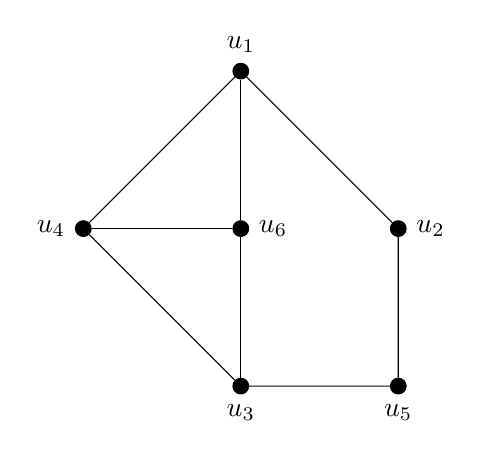
\begin{tikzpicture}
  \node[circle, draw, fill, inner sep=2pt, label=above:$u_1$] (u1) at (0,2) {};
  \node[circle, draw, fill, inner sep=2pt, label=right:$u_2$] (u2) at (2,0) {};
  \node[circle, draw, fill, inner sep=2pt, label=below:$u_3$] (u3) at (0,-2) {};
  \node[circle, draw, fill, inner sep=2pt, label=left:$u_4$] (u4) at (-2,0) {};
  \node[circle, draw, fill, inner sep=2pt, label=below:$u_5$] (u5) at (2,-2) {};
  \node[circle, draw, fill, inner sep=2pt, label=right:$u_6$] (u6) at (0,0) {};
  \draw (u1)--(u2)--(u5)--(u3)--(u4)--(u1);
  \draw (u1)--(u6)--(u3);
  \draw (u4)--(u6);
\end{tikzpicture}
\vspace{5mm}

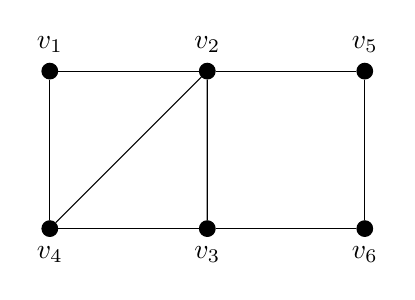
\begin{tikzpicture}
    \node[circle, draw, fill, inner sep=2pt, label=above:$v_1$] (v1) at (0,0) {};
  \node[circle, draw, fill, inner sep=2pt, label=above:$v_2$] (v2) at (2,0) {};
  \node[circle, draw, fill, inner sep=2pt, label=below:$v_3$] (v3) at (2,-2) {};
  \node[circle, draw, fill, inner sep=2pt, label=below:$v_4$] (v4) at (0,-2) {};
  \node[circle, draw, fill, inner sep=2pt, label=above:$v_5$] (v5) at (4,0) {};
  \node[circle, draw, fill, inner sep=2pt, label=below:$v_6$] (v6) at (4,-2) {};
   \draw (v1)--(v2)--(v5)--(v6)--(v3)--(v4)--(v1);
   \draw (v4)--(v2)--(v3);

\end{tikzpicture}
\end{parts}

\question WEEK 15 QUIZ
\begin{parts}
\part The given graph represents the classrooms at school and the paths that connect them together.
Your teacher asks you to go along all the paths to make sure they are clean and tidy, but you only have a
few minutes before the start of class so you can’t go over any path twice.\\
1. What kind of path are you looking for? Euler/Hamilton\\
2. Can you find a path through the graph?\\
3. Can you find a circuit? (It might not have one)
    \begin{figure}[htp]
    \centering
    \includegraphics[width=15cm]{puzzle.png}
    \caption{This graph represents the classrooms at school and the paths that connect them together.}
    \label{fig:galaxy}
\end{figure}
\end{parts}
\end{questions}
\end{document}
